%%%%%%%%%%%%%%%%%%%%%%%%%%%%%%%%%%%%%%%%%%%%%%%%%%%%%%%%%%%%%%%%%%%%%%%%%%%%%%%%%%%%%%%%%%%%%%%%%%%%%%%%%%%%%%%%%%%%%%%%%%%%%%%%%%%%%%%%%%%%%%%%%%%%%%%%%%%%%%%%%%%%%%%%%%%%%%%%%%%%
\section{Characterisation and estimation of the Standard Model backgrounds}
\label{sec:BackgroundEstimation}
After the application of the candidate track selection explained in the previous section the background arising from Standard Model processes is dramatically reduced.
However, it still happens sometimes that a electron, muon or tau fails reconstruction, which will be explained in detail in the following section~\ref{sec:LeptonicBkg}.
Furthermore, there is the possibility that a track is reconstructed out of a set of hits which do not origin from only one single particle.
Such tracks will be called ``fake tracks'' in the following. 
Background tracks arising from wrong reconstruction will be explained in Sec.~\ref{sec:FakeBkg}

The composition of the background is shown in Fig.~\ref{blabla}.
\begin{figure}[!tb]
  \centering 
  \begin{tabular}{c}
    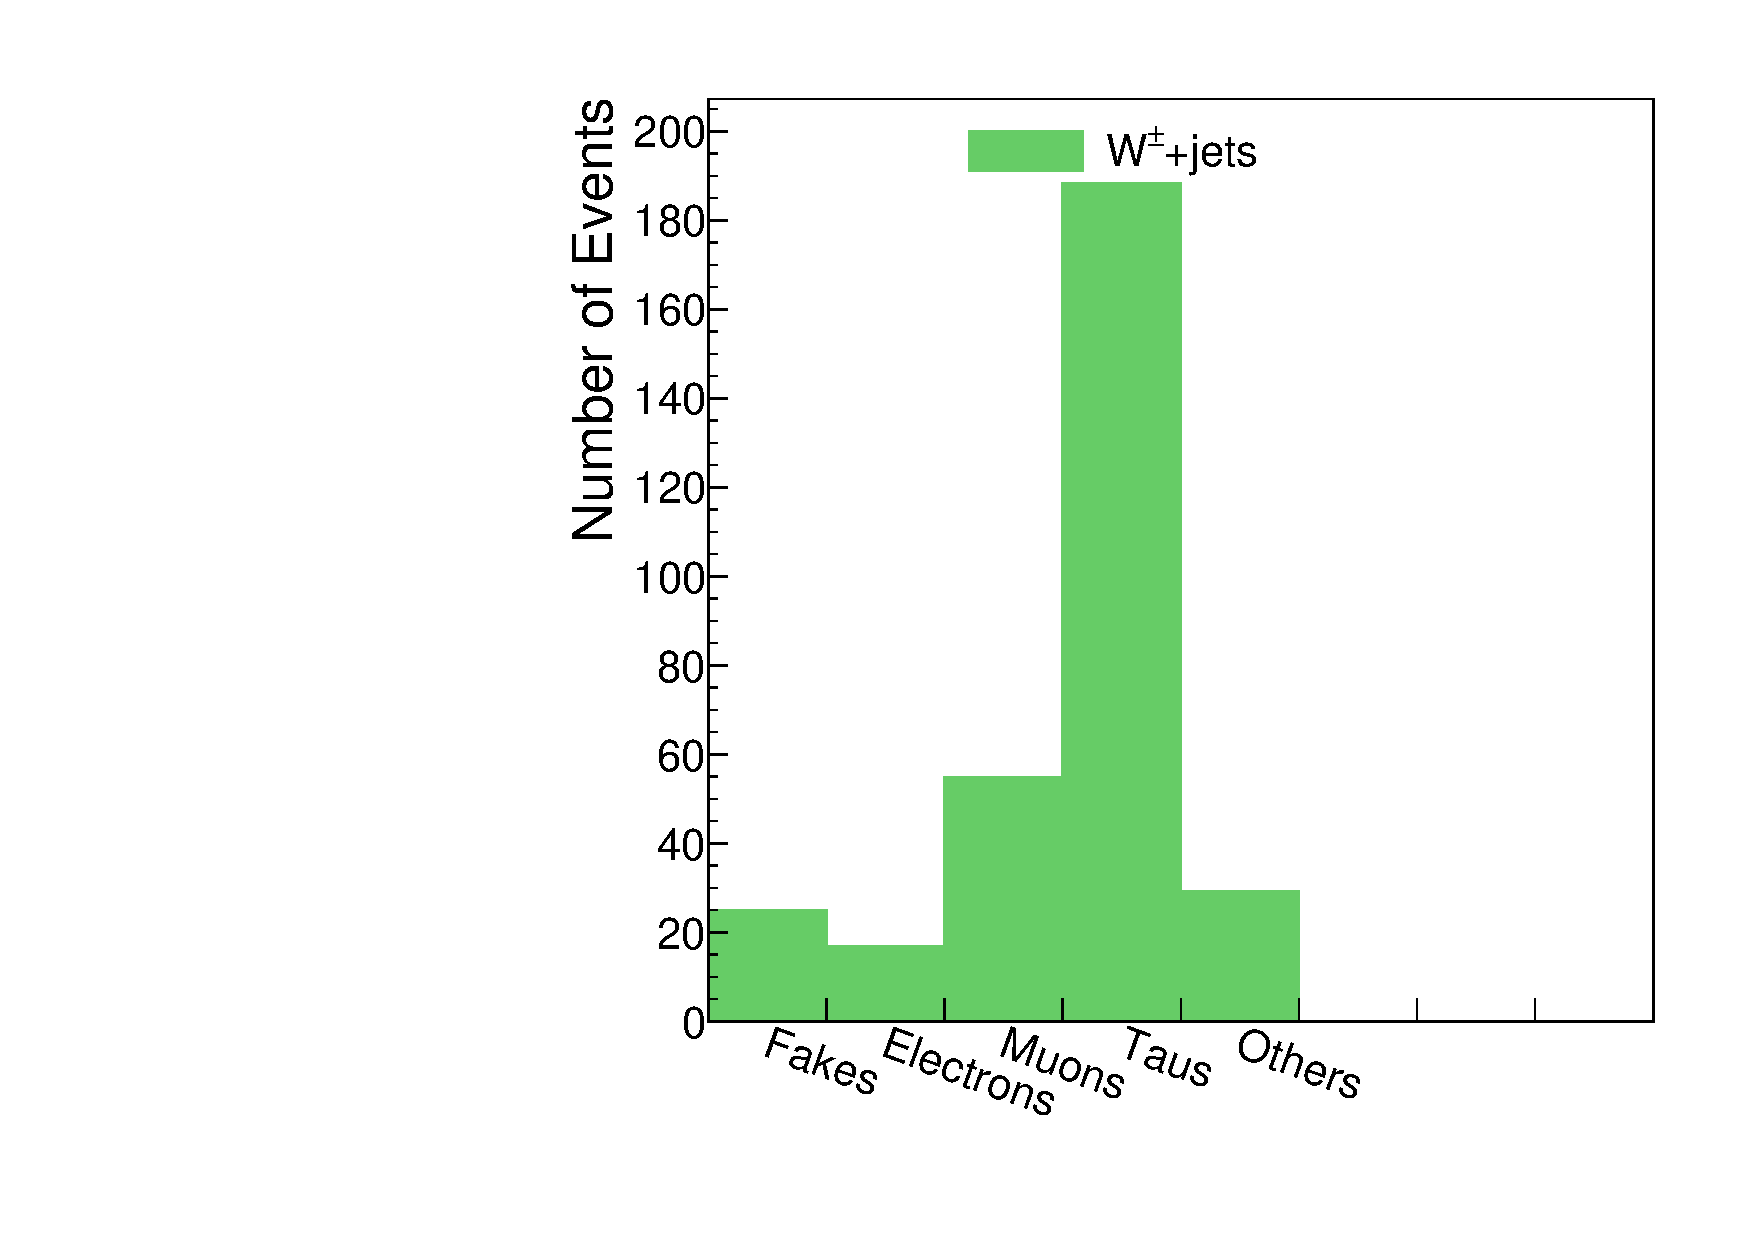
\includegraphics[width=0.49\textwidth]{figures/analysis/htrackgenParticleSmallRange_lin.pdf}
    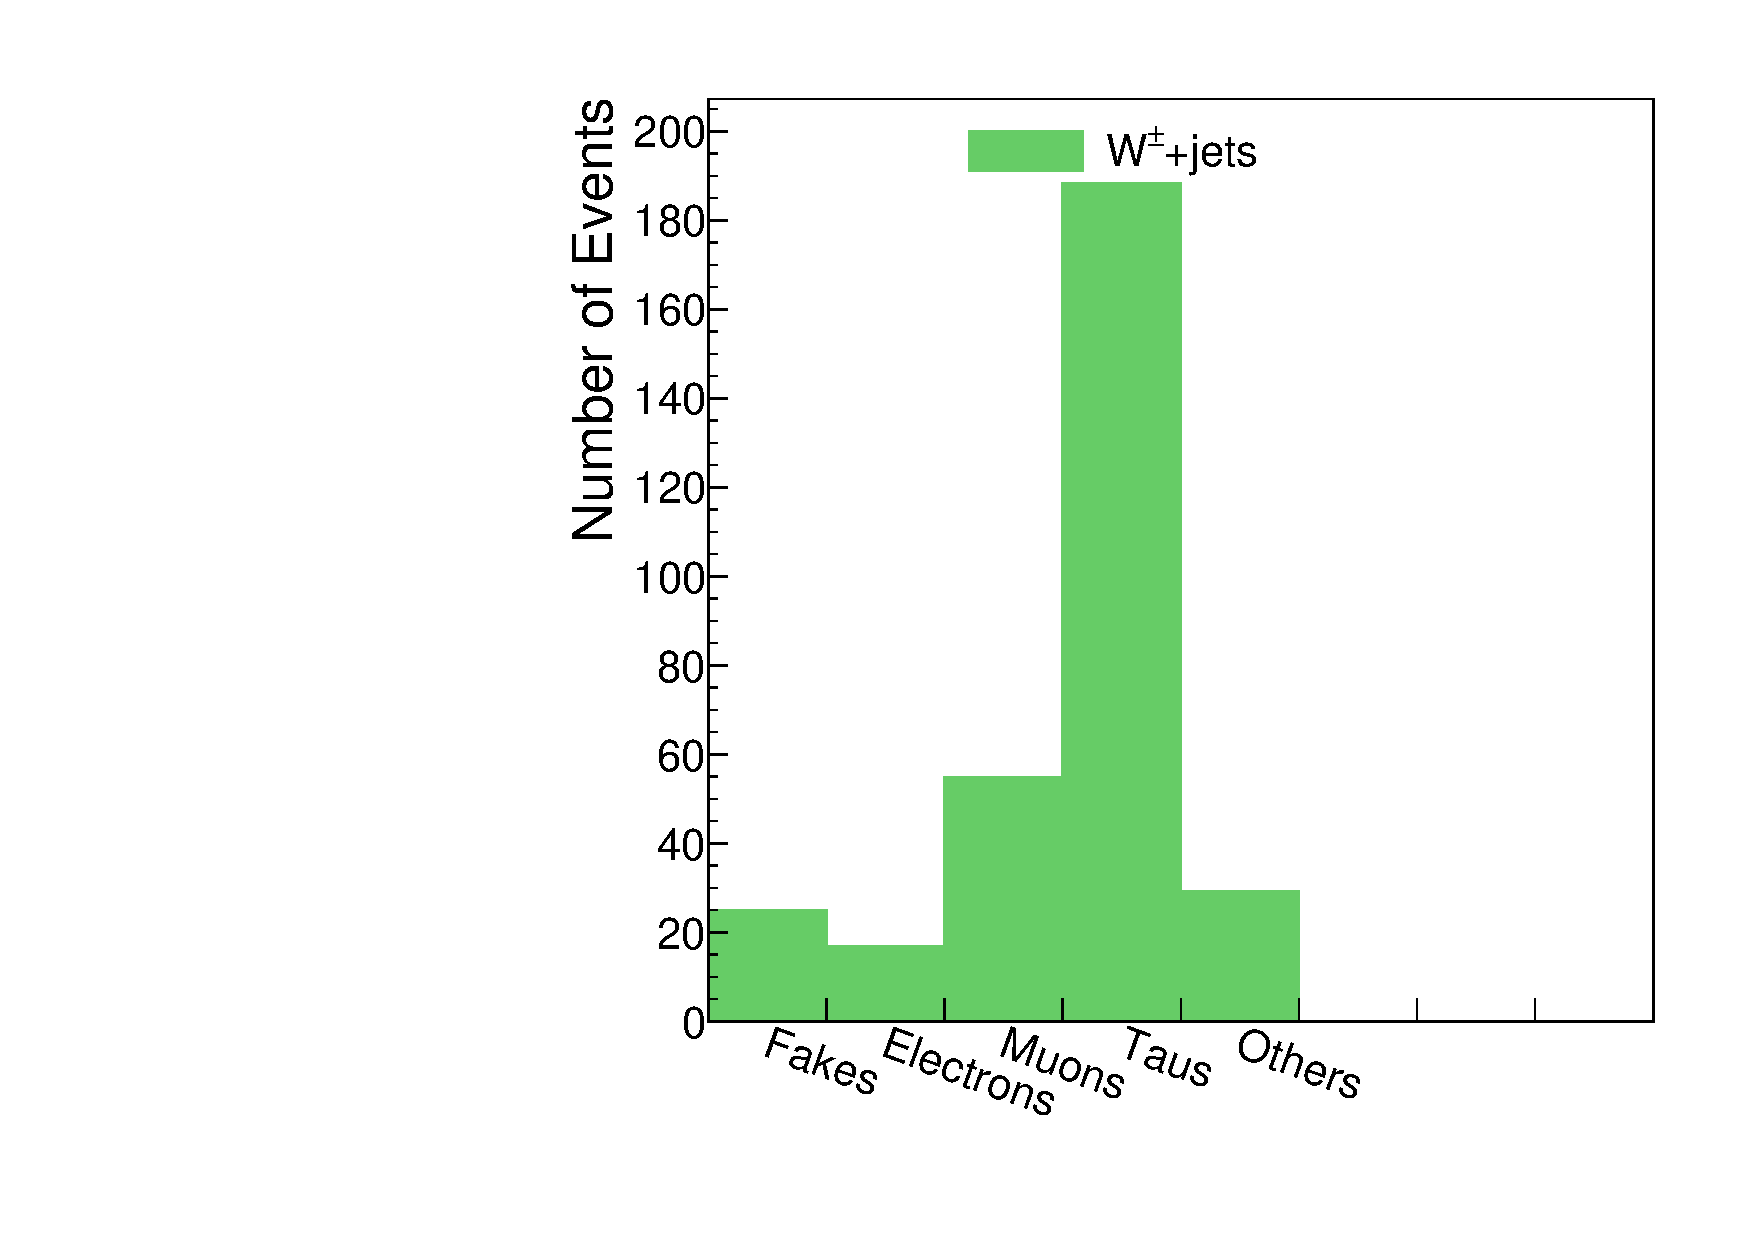
\includegraphics[width=0.49\textwidth]{figures/analysis/htrackgenParticleSmallRange_lin.pdf}
  \end{tabular}
  \caption{Candidate track \pt (left) and \ias (right) after the full candidate track selection for signal and $\WJets$ events. 
           Because of high event weights of the $\WJets$ sample, the \met and \ptfirstjet cuts are loosen to $\met>0\gev$ and $\ptfirstjet>70\gev$. 
           As these variables are not expected to be correlated with the track charecteristics it does not incluences the shape of the shown distributions.}
  \label{fig:PtAndIasAfterFullPreselection}
\end{figure}
This composiiton can change significantly when imposing further selection cuts on \pt and \ias.
This, however, is addresses within the optimisation.
To get a feeling how the composition can chnage, the bkg composition is shown in Fig~\ref{blabla} with the analysis selection plus an additional \ias cut of 0.5.


\begin{itemize}
\item Show plots with different selection cuts: after candidate track selection + ecalo$<$5\gev, 
\item Explain why we need data based approach
\item Explain that we cannot know before how important the leptonic bkg is.
\end{itemize}

\subsection{Leptonic background}
\label{sec:LeptonicBkg}

The leptonic background can arise from various sources: First, ...

\begin{itemize}
\item Characterization - describe shortly why a background can contribute
\item Electron: Explain again, that most of the preselection cuts are done for electrons
\item 
\end{itemize}


\subsection{Fake background}
\label{sec:FakeBkg}

\begin{itemize}
\item Show plot with fake rate in different samples
\end{itemize}

\subsection{Systematic uncertainties}
\label{sec:SysUncertaintiesBkg}


\begin{itemize}
\item Background consist of particles which make high energy deposits and are high pt
\item In general: Low background search
\end{itemize}


\newpage
%%%%%%%%%%%%%%%%%%%%%%%%%%%%%%%%%%%%%%%%%%%%%%%%%%%%%%%%%%%%%%%%%%%%%%%%%%%%%%%%%%%%%%%%%%%%%%%%%%%%%%%%%%%%%%%%%%%%%%%%%%%%%%%%%%%%%%%%%%%%%%%%%%%%%%%%%%%%%%%%%%%%%%%%%%%%%%%%%%%%
%%%%%%%%%%%%%%%%%%%%%%%%%%%%%%%%%%%%%%%%%%%%%%%%%%%%%%%%%%%%%%%%%%%%%%%%%%%%%%%%%%%%%%%%%%%%%%%%%%%%%%%%%%%%%%%%%%%%%%%%%%%%%%%%%%%%%%%%%%%%%%%%%%%%%%%%%%%%%%%%%%%%%%%%%%%%%%%%%%%%
\section{Optimization of search sensitivity}
\label{sec:Optimization}
\begin{itemize}
\item Show plots
\item show table
\item Include NlostOuter here, too
\end{itemize}

%%%%%%%%%%%%%%%%%%%%%%%%%%%%%%%%%%%%%%%%%%%%%%%%%%%%%%%%%%%%%%%%%%%%%%%%%%%%%%%%%%%%%%%%%%%%%%%%%%%%%%%%%%%%%%%%%%%%%%%%%%%%%%%%%%%%%%%%%%%%%%%%%%%%%%%%%%%%%%%%%%%%%%%%%%%%%%%%%%%%
\section{Statistical Methods/ Limit setting}
\label{sec:LimitSetting}

%%%%%%%%%%%%%%%%%%%%%%%%%%%%%%%%%%%%%%%%%%%%%%%%%%%%%%%%%%%%%%%%%%%%%%%%%%%%%%%%%%%%%%%%%%%%%%%%%%%%%%%%%%%%%%%%%%%%%%%%%%%%%%%%%%%%%%%%%%%%%%%%%%%%%%%%%%%%%%%%%%%%%%%%%%%%%%%%%%%%
\section{Results}
\label{sec:Results}
\begin{itemize}
\item Data cutflowtable
\item Tables with results
\item One plot (4 bins: Prediction and data)
\end{itemize}

%%%%%%%%%%%%%%%%%%%%%%%%%%%%%%%%%%%%%%%%%%%%%%%%%%%%%%%%%%%%%%%%%%%%%%%%%%%%%%%%%%%%%%%%%%%%%%%%%%%%%%%%%%%%%%%%%%%%%%%%%%%%%%%%%%%%%%%%%%%%%%%%%%%%%%%%%%%%%%%%%%%%%%%%%%%%%%%%%%%%
\section{Interpretation}
\label{sec:Interpretation}
\subsection{Systematic uncertainties of simulated signal samples}
\subsection{Exclusion limits}
\begin{itemize}
\item 1-d limits
\item 2-d limits
\end{itemize}

